\documentclass[braun, twocolumn]{braun}
\title{Entalpia}
\affiliation{Colégio e Curso Pensi, Coordenação de Química}
\author{Gabriel Braun}
\logo{pensi}
\dbpath{../database}

\begin{document}
\maketitle
\section{Nível I}


\begin{problem}
[2A01]\textbf{Assinale} a alternativa que mais se aproxima do valor absoluto
do trabalho realizado por um gás que se expande em \(\qty{500}{mL}\)
contra uma pressão de \(\qty{1,2}{atm}\).


\begin{choices}
(3)
\item \(\qty{54}{J}\)

\item \(\qty{60}{J}\)

\item \(\qty{66}{J}\)

\item \(\qty{72}{J}\)

\item \(\qty{70}{J}\)

\end{choices}

\end{problem}



\begin{problem}
[2A02]\textbf{Assinale} a alternativa que mais se aproxima do valor absoluto
do trabalho realizado no congelamento de \(\qty{100}{g}\) de água a
\(\qty{0}{\degree C}\) e \(\qty{1070}{atm}\).


\begin{choices}
(3)
\item \(\qty{720}{J}\)

\item \(\qty{790}{J}\)

\item \(\qty{860}{J}\)

\item \(\qty{880}{J}\)

\item \(\qty{910}{J}\)

\end{choices}

\end{problem}



\begin{problem}
[2A03]\textbf{Assinale} a alternativa que mais se aproxima do valor absoluto
do trabalho realizado quando \(\qty{50}{g}\) de ferro reagem com ácido
clorídrico formando gás hidrogênio e \(\ce{cloreto de ferro (II)}\) a
\(\qty{25}{\degree C}\).


\begin{choices}
(3)
\item \(\qty{2,2}{kJ}\)

\item \(\qty{4,4}{kJ}\)

\item \(\qty{6,6}{kJ}\)

\item \(\qty{8,8}{kJ}\)

\item \(\qty{5,3}{kJ}\)

\end{choices}

\end{problem}



\begin{problem}
[2A04]\textbf{Assinale} a alternativa que mais se aproxima do valor absoluto
do trabalho realizado na eletrólise de \(\qty{50}{g}\) de água formando
gás hidrogênio e oxigênio a \(\qty{25}{\degree C}\).


\begin{choices}
(3)
\item \(\qty{10}{kJ}\)

\item \(\qty{12}{kJ}\)

\item \(\qty{18}{kJ}\)

\item \(\qty{15}{kJ}\)

\item \(\qty{20}{kJ}\)

\end{choices}

\end{problem}



\begin{problem}
[2A05]Em um calorímetro foram adicionados \(\qty{20}{g}\) de um metal a
\(\qty{100}{\degree C}\) e \(\qty{50}{g}\) de água a \(\qty{22}{\degree C}\).
A temperatura final registrada foi \(\qty{25}{\degree C}\).

\textbf{Assinale} a alternativa que mais se aproxima da capacidade
calorífica do metal.


\begin{choices}
(2)
\item \(\qty{0,1}{J.K^{-1}.g^{-1}}\)

\item \(\qty{0,2}{J.K^{-1}.g^{-1}}\)

\item \(\qty{0,3}{J.K^{-1}.g^{-1}}\)

\item \(\qty{0,4}{J.K^{-1}.g^{-1}}\)

\item \(\qty{0,5}{J.K^{-1}.g^{-1}}\)

\end{choices}

\end{problem}



\begin{problem}
[2A06]Em um calorímetro adiabático foram adicionados \(\qty{300}{g}\) de gelo a
\(\qty{0}{\degree C}\) e \(\qty{400}{g}\) de água a \(\qty{55}{\degree C}\).

\textbf{Assinale} a alternativa que mais se aproxima da temperatura
final do sistema.


\begin{choices}
(3)
\item \(\qty{-4}{\degree C}\)

\item \(\qty{-3}{\degree C}\)

\item \(\qty{0}{\degree C}\)

\item \(\qty{3}{\degree C}\)

\item \(\qty{4}{\degree C}\)

\end{choices}
\subsubsection*{Dados}


\begin{datalist}

\item $\Delta H_\text{f}(\ce{H2O, {s}}) = \qty{-291,83}{kJ.mol^{-1}}$
\item $C_P(\ce{H2O, {s}}) = \qty{37,84}{J.K^{-1}.mol^{-1}}$
\item $C_P(\ce{H2O, {l}}) = \qty{75,29}{J.K^{-1}.mol^{-1}}$
\end{datalist}

\end{problem}



\begin{problem}
[2A07]A expansão de um gás ideal em um recipiente de \(\qty{1}{L}\) a
\(\qty{10}{atm}\) é realizada de duas maneiras diferentes em temperatura
constante.

\begin{enumerate}
\def\labelenumi{\arabic{enumi}.}

\item
  Expansão contra pressão constante de \(\qty{1}{atm}\), levando o volume
  final do recipiente a \(\qty{10}{L}\).
\item
  Expansão contra pressão constante de \(\qty{5}{atm}\) até atingir um
  volume de \(\qty{2}{L}\), seguida de expansão contra pressão constante
  de \(\qty{1}{atm}\) atingindo o volume final de \(\qty{10}{L}\).
\end{enumerate}

\textbf{Assinale} a alternativa \emph{correta}.


\begin{choices}

\item O trabalho realizado pelo gás é igual nos dois processos de expansão.

\item O trabalho realizado no primeiro processo é metade do trabalho realizado
no segundo processo.

\item A variação de energia interna do gás é igual em ambos os processos.

\item A variação de energia interna do gás no primeiro processo é metade da do
segundo processo.

\item O calor trocado pelo gás é igual em ambos os processos.

\end{choices}

\end{problem}



\begin{problem}
[2A08]Considere os processos químicos realizados em temperatura constante.

\begin{enumerate}
\def\labelenumi{\arabic{enumi}.}

\item
  Dissolução do nitrato de potássio.
\item
  Ebulição da água.
\item
  Conversão da grafita em diamante.
\item
  Oxidação do sódio metálico.
\end{enumerate}

\textbf{Assinale} a alternativa com os processos que apresentam variação
de energia interna não nula.


\begin{choices}
(3)
\item 1, 2 e 3

\item 1, 2 e 4

\item 1, 3 e 4

\item 2, 3 e 4

\item 1, 2, 3 e 3

\end{choices}

\end{problem}



\begin{problem}
[2A09]São descritos abaixo dois experimentos em que há sublimação completa de
uma mesma quantidade de dióxido de carbono no estado sólido a
\(\qty{25}{\degree C}\):

\begin{enumerate}
\def\labelenumi{\arabic{enumi}.}

\item
  O processo é realizado em um recipiente hermeticamente fechado, de
  paredes rígidas e indeformáveis.
\item
  O processo é realizado em cilindro provido de um pistão, cuja massa e
  desprezível e se desloca sem atrito.
\end{enumerate}

\textbf{Assinale} a alternativa \emph{incorreta}.


\begin{choices}

\item O primeiro processo ocorre com absorção de calor.

\item O valor absoluto do trabalho realizado é maior no primeiro.

\item A variação de energia interna é maior no primeiro processo.

\item Há realização de trabalho no segundo processo.

\item A variação de energia interna é igual ao calor no segundo processo.

\end{choices}

\end{problem}



\begin{problem}
[2A10]Um sistema termicamente isolado é composto por dois balões idênticos
resistentes, porém não inquebráveis, \textbf{A} e \textbf{B}, conectados
por um tubo com uma válvula fechada. O balão \textbf{A} contém um mol de
um gás ideal monoatômico e \textbf{B} encontra-se perfeitamente
evacuado. Em um dado instante a válvula é aberta.

\textbf{Assinale} a alternativa \emph{correta}.


\begin{choices}

\item O balão B quebrar-se-á devido ao impacto do gás ideal.

\item O trabalho gerado pela expansão do gás aquecerá o sistema.

\item O gás em expansão absorverá calor da vizinhança, resfriando o sistema.

\item A variação da energia interna da expansão será nula.

\item A variação da energia interna do sistema será negativa.

\end{choices}

\end{problem}



\begin{problem}
[2A11]\textbf{Assinale} a alternativa que mais se aproxima da variação de
entalpia quando um mol de um gás pressurizado em \(\qty{1}{MPa}\) e
\(\qty{300}{K}\) se expande adiabaticamente contra pressão de
\(\qty{0,1}{MPa}\) até atingir o equilíbrio.


\begin{choices}
(3)
\item \(\qty{15}{kJ}\)

\item \(\qty{17}{kJ}\)

\item \(\qty{20}{kJ}\)

\item \(\qty{22}{kJ}\)

\item \(\qty{25}{kJ}\)

\end{choices}

\end{problem}



\begin{problem}
[2A12]\textbf{Assinale} a alternativa que mais se aproxima da variação de
entalpia quando \(\qty{500}{J}\) de energia são transferidos em volume
constante a uma amostra contendo \(\qty{0,9}{mol}\) de oxigênio.


\begin{choices}
(3)
\item \(\qty{-700}{J}\)

\item \(\qty{-500}{J}\)

\item \(\qty{300}{J}\)

\item \(\qty{500}{J}\)

\item \(\qty{700}{J}\)

\end{choices}
\subsubsection*{Dados}


\begin{datalist}

\item $C_P(\ce{O2, {g}}) = \qty{29,36}{J.K^{-1}.mol^{-1}}$
\end{datalist}

\end{problem}



\begin{problem}
[2A13]Considere a curva de aquecimento para uma substância sólida com apenas
uma fase cristalina.

\begin{figure}
\centering
\includegraphics{images/2A13-1P.svg}
\caption{Temperatura por tempo.}
\end{figure}

Considere as proposições.

\textbf{Assinale} a alternativa que relaciona as proposições
\emph{incorretas}.


\begin{choices}

\item Na região entre \emph{P} e \emph{Q} ocorre aumento da energia cinética.

\item Na região entre \emph{Q} e \emph{R} ocorre aumento da energia potencial.

\item O calor de fusão da substância é menor que o seu calor de vaporização.

\item O calor específico do sólido é maior que o calor específico do líquido.

\end{choices}

\end{problem}



\begin{problem}
[2A14]Amostras de massas iguais de duas substâncias, \textbf{A} e \textbf{B},
foram submetidas independentemente a um processo de aquecimento em
atmosfera inerte e sob pressão constante. A curva de aquecimento das
amostras é apresentado a seguir.

\begin{figure}
\centering
\includegraphics{images/2A14-1P.svg}
\caption{Temaperatura por calor trocado.}
\end{figure}

\textbf{Assinale} a alternativa \emph{incorreta}.


\begin{choices}

\item A entalpia de fusão de \textbf{A} é menor que a de \textbf{B}.

\item A entalpia de vaporização de \textbf{A} é menor que a de \textbf{B}.

\item A capacidade calorífica na fase sólida de \textbf{A} é menor que na de
\textbf{B}.

\item A capacidade calorífica na fase líquida de \textbf{A} é maior que na de
\textbf{B}.

\item A capacidade calorífica na fase gasosa de \textbf{A} é maior que na de
\textbf{B}.

\end{choices}

\end{problem}



\begin{problem}
[2A15]Considera a variação da capacidade calorífica de uma substância com a
temperatura.

\begin{figure}
\centering
\includegraphics{images/2A15-1P.svg}
\caption{CP por temperatura.}
\end{figure}

\textbf{Assinale} a alternativa \emph{incorreta}.


\begin{choices}

\item A substância apresenta mais de uma estrutura cristalina.

\item A capacidade calorífica da substância é menor no estado gasoso do que no
estado líquido.

\item A capacidade calorífica para qualquer fase da substância aumenta com o
aumento da temperatura.

\item Caso a substância se mantenha no estado líquido em temperaturas
inferiores a \(T_f\), a capacidade calorífica da substância líquida é
maior que a capacidade calorífica da fase sólida metaestável em
temperaturas inferiores à \(T_f\).

\item A variação de entalpia quando essa substância sofre uma reação química
no estado líquido aumenta com o aumento da temperatura.

\end{choices}

\end{problem}



\begin{problem}
[2A16]Aminoácidos são oxidata: no organismo formando ureia
(\(\ce{H2NCONH2}\)), dióxido de carbono e água.

\textbf{Assinale} a alternativa do valor mais próximo da entalpia de
oxidação da glicina (\(\ce{NH2CH2COOH}\)).


\begin{choices}
(2)
\item \(\qty{620}{kJ.mol^{-1}}\)

\item \(\qty{650}{kJ.mol^{-1}}\)

\item \(\qty{680}{kJ.mol^{-1}}\)

\item \(\qty{710}{kJ.mol^{-1}}\)

\item \(\qty{740}{kJ.mol^{-1}}\)

\end{choices}
\subsubsection*{Dados}


\begin{datalist}

\item $\Delta H_\text{f}(\ce{ureia, {s}}) = \qty{-333,51}{kJ.mol^{-1}}$
\item $\Delta H_\text{f}(\ce{CO2, {g}}) = \qty{-393,51}{kJ.mol^{-1}}$
\item $\Delta H_\text{f}(\ce{H2O, {l}}) = \qty{-285,83}{kJ.mol^{-1}}$
\end{datalist}

\end{problem}



\begin{problem}
[2A17]\textbf{Assinale} a alternativa que mais se aproxima da entalpia de
formação do metano.


\begin{choices}
(2)
\item \(\qty{-225}{kJ.mol^{-1}}\)

\item \(\qty{-75}{kJ.mol^{-1}}\)

\item \(\qty{75}{kJ.mol^{-1}}\)

\item \(\qty{150}{kJ.mol^{-1}}\)

\item \(\qty{225}{kJ.mol^{-1}}\)

\end{choices}
\subsubsection*{Dados}


\begin{datalist}

\item $\Delta H_\text{f}(\ce{CO2, {g}}) = \qty{-393,51}{kJ.mol^{-1}}$
\item $\Delta H_\text{f}(\ce{H2O, {g}}) = \qty{-241,82}{kJ.mol^{-1}}$
\item $\Delta H_\text{c}(\ce{CH4, {g}}) = \qty{-890}{kJ.mol^{-1}}$
\end{datalist}

\end{problem}



\begin{problem}
[2A18]\textbf{Assinale} a alternativa que mais se aproxima da razão entre a
energia liberada por átomo de hidrogênio na combustão completa do octano
gasoso e na célula de combustível de hidrogênio e oxigênio.


\begin{choices}
(5)
\item \(0,2\)

\item \(0,5\)

\item \(1,0\)

\item \(2,5\)

\item \(5,0\)

\end{choices}
\subsubsection*{Dados}


\begin{datalist}

\item $\Delta H_\text{L}(\ce{C-C}) = \qty{348}{kJ.mol^{-1}}$
\item $\Delta H_\text{L}(\ce{C-H}) = \qty{412}{kJ.mol^{-1}}$
\item $\Delta H_\text{L}(\ce{C=O}) = \qty{743}{kJ.mol^{-1}}$
\item $\Delta H_\text{L}(\ce{H2}) = \qty{436}{kJ.mol^{-1}}$
\item $\Delta H_\text{L}(\ce{O2}) = \qty{496}{kJ.mol^{-1}}$
\end{datalist}

\end{problem}



\begin{problem}
[2A19]\textbf{Assinale} a alternativa que mais se aproxima da entalpia de
bromação de um mol de \(\ce{propeno}\) (\(\ce{CH3CHCH2}\)), formando
\(\ce{1,2-dibromopropano}\)
(\(\ce{CH3CHBrCH2Br}, \Delta H_\text{vap} = \pu{35.61 kJ.mol^{-1}}\)).


\begin{choices}
(3)
\item \(\qty{-101}{kJ}\)

\item \(\qty{-401}{kJ}\)

\item \(\qty{-302}{kJ}\)

\item \(\qty{-130}{kJ}\)

\item \(\qty{-202}{kJ}\)

\end{choices}
\subsubsection*{Dados}


\begin{datalist}

\item $\Delta H_\text{vap}(\ce{Br2}) = \qty{30,91}{kJ.mol^{-1}}$
\item $\Delta H_\text{L}(\ce{C=C}) = \qty{612}{kJ.mol^{-1}}$
\item $\Delta H_\text{L}(\ce{Br2}) = \qty{193}{kJ.mol^{-1}}$
\end{datalist}

\end{problem}



\begin{problem}
[2A20]\textbf{Assinale} a alternativa que mais se aproxima da entalpia de
formação do metanol.


\begin{choices}
(2)
\item \(\qty{-260}{kJ.mol^{-1}}\)

\item \(\qty{-200}{kJ.mol^{-1}}\)

\item \(\qty{-130}{kJ.mol^{-1}}\)

\item \(\qty{130}{kJ.mol^{-1}}\)

\item \(\qty{260}{kJ.mol^{-1}}\)

\end{choices}
\subsubsection*{Dados}


\begin{datalist}

\item $\Delta H_\text{sub}(\ce{grafite}) = \qty{712}{kJ.mol^{-1}}$
\item $\Delta H_\text{L}(\ce{H2}) = \qty{436}{kJ.mol^{-1}}$
\item $\Delta H_\text{L}(\ce{O2}) = \qty{496}{kJ.mol^{-1}}$
\item $\Delta H_\text{L}(\ce{C-H}) = \qty{412}{kJ.mol^{-1}}$
\item $\Delta H_\text{L}(\ce{C-O}) = \qty{360}{kJ.mol^{-1}}$
\item $\Delta H_\text{L}(\ce{O-H}) = \qty{463}{kJ.mol^{-1}}$
\end{datalist}

\end{problem}



\begin{problem}
[2A21]A hidrogenação do monóxido de carbono libera \(\qty{131}{kJ}\) por mol de
grafita formado.

\textbf{Assinale} a alternativa que mais se aproxima da entalpia de
reforma de \(\qty{1}{mol}\) de metano com vapor d'água, método industrial
para produção de hidrogênio.


\begin{choices}
(2)
\item \(\qty{+207}{kJ.mol^{-1}}\)

\item \(\qty{-204}{kJ.mol^{-1}}\)

\item \(\qty{+302}{kJ.mol^{-1}}\)

\item \(\qty{-197}{kJ.mol^{-1}}\)

\item \(\qty{+250}{kJ.mol^{-1}}\)

\end{choices}
\subsubsection*{Dados}


\begin{datalist}

\item $\Delta H_\text{f}(\ce{CO2, {g}}) = \qty{-393,51}{kJ.mol^{-1}}$
\item $\Delta H_\text{f}(\ce{H2O, {l}}) = \qty{-285,83}{kJ.mol^{-1}}$
\item $\Delta H_\text{c}(\ce{CH4, {g}}) = \qty{-890}{kJ.mol^{-1}}$
\end{datalist}

\end{problem}



\begin{problem}
[2A22]\textbf{Assinale} a alternativa que mais se aproxima da entalpia de
desidrogenação de \(\qty{1}{mol}\) de propano, formando propeno.


\begin{choices}
(2)
\item \(\qty{-3,5}{MJ}\)

\item \(\qty{-2,2}{MJ}\)

\item \(\qty{+2,2}{MJ}\)

\item \(\qty{+125,4}{kJ}\)

\item \(\qty{+114,0}{kJ}\)

\end{choices}
\subsubsection*{Dados}


\begin{datalist}

\item $\Delta H_\text{f}(\ce{propeno, {g}}) = \qty{20,42}{kJ.mol^{-1}}$
\item $\Delta H_\text{f}(\ce{CO2, {g}}) = \qty{-393,51}{kJ.mol^{-1}}$
\item $\Delta H_\text{c}(\ce{propano, {g}}) = \qty{-2220}{kJ.mol^{-1}}$
\end{datalist}

\end{problem}



\begin{problem}
[2A23]Uma amostra de \(\qty{0,113}{g}\) de benzeno é queimada em um calorímetro
isobárico (C = \(\qty{551}{J.\degree C^{-1}}\)) com excesso de oxigênio. A
elevação de temperatura registrada foi de \(\qty{8,60}{\degree C}\).

\textbf{Assinale} a alternativa que mais se aproxima da entalpia de
combustão do benzeno.


\begin{choices}
(3)
\item \(\qty{-6,55}{MJ}\)

\item \(\qty{-7,05}{MJ}\)

\item \(\qty{-8,90}{MJ}\)

\item \(\qty{-5,50}{MJ}\)

\item \(\qty{-9,75}{MJ}\)

\end{choices}

\end{problem}



\begin{problem}
[2A24]Um calorímetro foi calibrado pela queima de \(\qty{0,825}{g}\) de ácido
benzoico com excesso de oxigênio. A elevação de temperatura registrada
foi de \(\qty{8,60}{\degree C}\). Quando uma amostra com \(\qty{0,725}{g}\)
de ribose (\(\ce{C5H10O5}\)) é queimada no mesmo calorímetro, a
temperatura aumenta de \(\qty{21,81}{\degree C}\) para
\(\qty{22,72}{\degree C}\).

\textbf{Assinale} a alternativa que mais se aproxima da energia de
combustão da ribose.


\begin{choices}
(2)
\item \(\qty{220}{kJ.mol^{-1}}\)

\item \(\qty{4700}{kJ.mol^{-1}}\)

\item \(\qty{580}{kJ.mol^{-1}}\)

\item \(\qty{740}{kJ.mol^{-1}}\)

\item \(\qty{850}{kJ.mol^{-1}}\)

\end{choices}
\subsubsection*{Dados}


\begin{datalist}

\item $\Delta H_\text{c}(\ce{C6H5COOH, {s}}) = \qty{-3227}{kJ.mol^{-1}}$
\end{datalist}

\end{problem}



\begin{problem}
[2A25]Uma amostra de \(\qty{1}{mol}\) de glicose é queimada em um calorímetro
isocórico (\(C = \qty{512}{J.\degree C^{-1}}\)) com excesso de oxigênio. A
variação de temperatura registrada foi de \(\qty{5}{\degree C}\).

\textbf{Assinale} a alternativa que mais se aproxima da entalpia de
combustão da glicose.


\begin{choices}
(2)
\item \(\qty{-2575}{kJ}\)

\item \(\qty{-2560}{kJ}\)

\item \(\qty{-2545}{kJ}\)

\item \(\qty{2545}{kJ}\)

\item \(\qty{2560}{kJ}\)

\end{choices}

\end{problem}



\begin{problem}
[2A26]Em um cilindro, provido de um pistão móvel sem atrito, é realizada a
combustão completa de carbono. A temperatura no interior do cilindro é
mantida constante desde a introdução dos reagentes até o final da
reação.

\begin{enumerate}
\def\labelenumi{\arabic{enumi}.}

\item
  A variação da energia interna do sistema é igual a zero.
\item
  O sistema não realiza trabalho.
\item
  A quantidade de calor trocada entre o sistema e a vizinhança é igual a
  zero.
\item
  A variação da entalpia do sistema é igual à variação da energia
  interna.
\end{enumerate}

\textbf{Assinale} a alternativa que relaciona as proposições corretas.


\begin{choices}
(3)
\item 1, 2 e 3

\item 1, 2 e 3

\item 1, 2 e 3

\item 1, 2 e 3

\item 1, 2 e 3

\end{choices}

\end{problem}



\begin{problem}
[2A27]\textbf{Assinale} a alternativa que mais se aproxima da massa de butano
necessária para aquecer \(\qty{1}{L}\) de água de \(\qty{17}{\degree C}\) a
\(\qty{100}{\degree C}\).

Resposta: {[}B{]}


\begin{choices}
(3)
\item \(\qty{3}{g}\)

\item \(\qty{7}{g}\)

\item \(\qty{14}{g}\)

\item \(\qty{21}{g}\)

\item \(\qty{28}{g}\)

\end{choices}
\subsubsection*{Dados}


\begin{datalist}

\item $\Delta H_\text{c}(\ce{butano, {g}}) = \qty{-2878}{kJ.mol^{-1}}$
\item $C_P(\ce{H2O, {l}}) = \qty{75,29}{J.K^{-1}.mol^{-1}}$
\item $\rho(\ce{H2O}) = \qty{1}{g.cm^{^{-3}}}$
\end{datalist}

\end{problem}



\begin{problem}
[2A28]O poder calorífico superior (PCS) e o poder calorífico inferior (PCI)
são definidos como a energia liberada na combustão completa de uma
substância formando água líquida e gasosa, respectivamente.

\textbf{Assinale} a alternativa que mais se aproxima do PCI do etanol
(\(\text{PCS} = \qty{30}{MJ.kg^{-1}}\)).


\begin{choices}
(2)
\item \(\qty{21}{MJ.kg^{-1}}\)

\item \(\qty{27}{MJ.kg^{-1}}\)

\item \(\qty{30}{MJ.kg^{-1}}\)

\item \(\qty{33}{MJ.kg^{-1}}\)

\item \(\qty{39}{MJ.kg^{-1}}\)

\end{choices}
\subsubsection*{Dados}


\begin{datalist}

\item $\Delta H_\text{vap}(\ce{H2O}) = \qty{40,7}{kJ.mol^{-1}}$
\end{datalist}

\end{problem}
\section{Nível II}


\begin{problem}
[2A29]Uma substância de massa molar \(\qty{200}{g.mol^{-1}}\) foi colocada em um
recipiente equipado com uma serpentina de aquecimento resistivo, a
\(\qty{80}{\degree C}\) e \(\qty{1}{bar}\). Para a manutenção da
temperatura, foi utilizada uma fonte de \(\qty{30}{V}\) e \(\qty{900}{mA}\)
durante \(\qty{30}{s}\), vaporizando \(\qty{2}{g}\) da substância.

\textbf{Assinale} a alternativa que mais se aproxima da entalpia de
vaporização dessa substância.


\begin{choices}
(2)
\item \(\qty{8}{kJ.mol^{-1}}\)

\item \(\qty{40}{kJ.mol^{-1}}\)

\item \(\qty{80}{kJ.mol^{-1}}\)

\item \(\qty{400}{kJ.mol^{-1}}\)

\item \(\qty{800}{kJ.mol^{-1}}\)

\end{choices}

\end{problem}



\begin{problem}
[2A30]Um calorímetro foi calibrado aplicando uma corrente de \(\qty{1}{A}\) de
uma fonte de \(\qty{9}{V}\) por \(\qty{150}{s}\), sendo registrada uma
variação de temperatura de \(\qty{5}{\degree C}\). Em um segundo
experimento, um mol de uma substância foi queimado nesse calorímetro e a
variação de temperatura registrada foi de \(\qty{3}{\degree C}\).

\textbf{Assinale} a alternativa que mais se aproxima da entalpia de
vaporização dessa substância.


\begin{choices}
(2)
\item \(\qty{510}{kJ.mol^{-1}}\)

\item \(\qty{610}{kJ.mol^{-1}}\)

\item \(\qty{710}{kJ.mol^{-1}}\)

\item \(\qty{810}{kJ.mol^{-1}}\)

\item \(\qty{910}{kJ.mol^{-1}}\)

\end{choices}

\end{problem}



\begin{problem}
[2A31]O perclorato de amônio (PA) é um dos componentes mais utilizados em
propelentes de foguetes. Para aperfeiçoar seu desempenho, hidrogênio
pode ser utilizado como aditivo. Considere o poder calorífico dessa
mistura em função da fração mássica de hidrogênio.

Fração mássica (\%) \textbar{} Poder calorífico (\(\unit{kJ.g^{-1}}\))
\textbar{} -\/-: \textbar{} -\/-: \textbar{} \(\num{2}\) \textbar{}
\(\num{3,0}\) \textbar{} \(\num{5}\) \textbar{} \(\num{8,7}\) \textbar{}

\begin{itemize}

\item
  \textbf{Determine} a entalpia de combustão do perclorato de amônio.
\item
  \textbf{Determine} a entalpia de combustão do hidrogênio.
\end{itemize}

\end{problem}



\begin{problem}
[2A32]Uma mistura de metano e eteno foi queimada em um reator de
\(\qty{3,0}{L}\) a \(\qty{25}{\degree C}\), em presença de excesso de
oxigênio. O reator é equipado com uma jaqueta externa, preenchida com
\(\qty{1}{L}\) de água, que mantém a temperatura constante em seu
interior. A combustão foi realizada a \(\qty{25}{\degree C}\), liberando
\(\qty{242,7}{kcal}\), e reduzindo a pressão em \(\qty{16,3}{atm}\).

\begin{itemize}

\item
  \textbf{Determine} a energia interna de combustão do metano e do
  eteno.
\item
  \textbf{Determine} a massa de metano na mistura inicial.
\end{itemize}
\subsubsection*{Dados}


\begin{datalist}

\item $C_P(\ce{H2O, {l}}) = \qty{75,29}{J.K^{-1}.mol^{-1}}$
\item $\Delta H_\text{f}(\ce{H2O, {l}}) = \qty{-285,83}{kJ.mol^{-1}}$
\item $\Delta H_\text{f}(\ce{CO2, {g}}) = \qty{-393,51}{kJ.mol^{-1}}$
\item $\Delta H_\text{f}(\ce{eteno, {g}}) = \qty{52,26}{kJ.mol^{-1}}$
\item $\Delta H_\text{f}(\ce{metano, {g}}) = \qty{-74,81}{kJ.mol^{-1}}$
\end{datalist}

\end{problem}



\begin{problem}
[2A33]\textbf{Determine} a energia liberada durante a precipitação
pluviométrica de \(\qty{20}{mm}\) de chuva sobre uma área de
\(\qty{100}{km2}\).
\subsubsection*{Dados}


\begin{datalist}

\item $\Delta H_\text{vap}(\ce{H2O}) = \qty{40,7}{kJ.mol^{-1}}$
\item $\rho(\ce{H2O}) = \qty{1}{g.cm^{^{-3}}}$
\end{datalist}

\end{problem}



\begin{problem}
[2A34]O consumo global anual de energia é cerca de \(\qty{100}{terawatts-ano}\),
sendo \(\pu{30\%}\) desse valor proveniente da queima de combustíveis
fósseis. Considere que os combustíveis fósseis são compostos
majoritariamente por octano, contendo \(\qty{10}{ppm}\) de enxofre. Apenas
\(\pu{80\%}\) da energia liberada na combustão completa pode ser
aproveitada.

\begin{itemize}

\item
  \textbf{Apresente} a reação de combustão completa do octano com ar
  atmosférico.
\item
  \textbf{Determine} a massa de dióxido de enxofre formada por hora
  devido à queima de combustíveis fósseis.
\end{itemize}
\subsubsection*{Dados}


\begin{datalist}

\item $\Delta H_\text{f}(\ce{H2O, {l}}) = \qty{-285,83}{kJ.mol^{-1}}$
\item $\Delta H_\text{f}(\ce{CO2, {g}}) = \qty{-393,51}{kJ.mol^{-1}}$
\item $\Delta H_\text{f}(\ce{octano, {l}}) = \qty{-249,9}{kJ.mol^{-1}}$
\end{datalist}

\end{problem}



\begin{problem}
[2A35]Considere os processos químicos a seguir.

\begin{enumerate}
\def\labelenumi{\arabic{enumi}.}

\item
  Reação de formação da água gasosa.
\item
  Reação de formação da água líquida.
\end{enumerate}

\textbf{Assinale} a alternativa \emph{incorreta}.


\begin{choices}

\item As reações \(1\) e \(2\) são exotérmicas.

\item O valor absoluto da variação de entalpia é menor que o da variação de
energia interna para a reação \(1\).

\item O valor absoluto da variação de energia interna da reação \(1\) é menor
que o da \(2\).

\item O valor absoluto da variação de entalpia da reação \(1\) é menor que o
da \(2\).

\item A capacidade calorífica do produto da reação \(1\) é menor que o da
\(2\).

\end{choices}

\end{problem}



\begin{problem}
[2A36]Considere os processos a seguir, em \(\qty{298}{K}\) e \(\qty{1}{atm}\).

Combustão de \(\qty{1}{g}\) de etanol formando fuligem. Combustão de
\(\qty{1}{g}\) de etanol formando monóxido de carbono.

\textbf{Assinale} a alternativa \emph{correta}.


\begin{choices}

\item Os processos ocorrem com a mesma variação de energia interna.

\item Os processos ocorrem com a mesma variação de entalpia.

\item O valor absoluto da variação de energia interna é maior para o primeiro
processo.

\item O valor absoluto da variação de entalpia é maior que o valor absoluto da
variação de energia interna para o primeiro processo.

\item O valor absoluto da variação de entalpia é menor que o valor absoluto da
variação de energia interna para o segundo processo.

\end{choices}

\end{problem}



\begin{problem}
[2A37]\textbf{Determine} a entalpia de combustão do octano.
\subsubsection*{Dados}


\begin{datalist}

\item $\Delta H_\text{c}(\ce{pentano, {g}}) = \qty{-3537}{kJ.mol^{-1}}$
\item $\Delta H_\text{c}(\ce{butano, {g}}) = \qty{-2878}{kJ.mol^{-1}}$
\end{datalist}

\end{problem}



\begin{problem}
[2A38]Amostras de \(\qty{5}{g}\) de etano e propano foram queimadas
independentemente em um calorímetro a \(\qty{298}{K}\) e \(\qty{1}{atm}\),
liberando \(\qty{260}{kJ}\) e \(\qty{250}{kJ}\) de energia, respectivamente.

\begin{itemize}

\item
  \textbf{Determine} a energia da ligação \(\ce{C-C}\).
\item
  \textbf{Determine} a energia da ligação \(\ce{C-H}\).
\end{itemize}
\subsubsection*{Dados}


\begin{datalist}

\item $\Delta H_\text{f}(\ce{CO2, {g}}) = \qty{-393,51}{kJ.mol^{-1}}$
\item $\Delta H_\text{sub}(\ce{grafite}) = \qty{712}{kJ.mol^{-1}}$
\item $\Delta H_\text{L}(\ce{H2}) = \qty{436}{kJ.mol^{-1}}$
\item $\Delta H_\text{f}(\ce{H2O, {l}}) = \qty{-285,83}{kJ.mol^{-1}}$
\end{datalist}

\end{problem}



\begin{problem}
[2A39]\textbf{Assinale} a alternativa que mais se aproxima da temperatura
adiabática de chama para a combustão octano líquido com \(\pu{300\%}\)
de excesso de ar atmosférico.


\begin{choices}
(3)
\item \(\qty{580}{K}\)

\item \(\qty{680}{K}\)

\item \(\qty{780}{K}\)

\item \(\qty{880}{K}\)

\item \(\qty{980}{K}\)

\end{choices}
\subsubsection*{Dados}


\begin{datalist}

\item $C_P(\ce{H2O, {g}}) = \qty{33,58}{J.K^{-1}.mol^{-1}}$
\item $C_P(\ce{CO2, {g}}) = \qty{37,11}{J.K^{-1}.mol^{-1}}$
\item $C_P(\ce{O2, {g}}) = \qty{29,36}{J.K^{-1}.mol^{-1}}$
\item $C_P(\ce{N2, {g}}) = \qty{29,12}{J.K^{-1}.mol^{-1}}$
\item $\Delta H_\text{f}(\ce{H2O, {g}}) = \qty{-241,82}{kJ.mol^{-1}}$
\item $\Delta H_\text{f}(\ce{CO2, {g}}) = \qty{-393,51}{kJ.mol^{-1}}$
\item $\Delta H_\text{f}(\ce{octano, {l}}) = \qty{-249,9}{kJ.mol^{-1}}$
\end{datalist}

\end{problem}



\begin{problem}
[2A40]Uma mistura (\(1:15\)) de metano e ar atmosférico, a \(\qty{298}{K}\) e
\(\qty{1}{atm}\), entra em combustão em um reservatório adiabático,
consumindo completamente o metano. O processo ocorre sob pressão
constante e os produtos formados permanecem em fase gasosa. Considere os
data: termodinâmicos a seguir.

\textbar{} \textbar{} \(\ce{H0}\)(\(\qty{1700}{K}\)) ---
\(\ce{H0}\)(\(\qty{298}{K}\)) \textbar{} \(\ce{H0}\)(\(\qty{2000}{K}\)) ---
\(\ce{H0}\)(\(\qty{298}{K}\)) \textbar{} \textbar{} :-\/- \textbar{} -\/-:
\textbar{} -\/-: \textbar{} \textbar{} \(\ce{CO2}\) \textbar{}
\(\qty{17,58}{kcal.mol^{-1}}\) \textbar{} \(\qty{21,90}{kcal/mol^{-1}}\)
\textbar{} \textbar{} \(\ce{H2O}\) \textbar{} \(\qty{13,74}{kcal.mol^{-1}}\)
\textbar{} \(\qty{17,26}{kcal.mol^{-1}}\) \textbar{} \textbar{} \(\ce{N2}\)
\textbar{} \(\qty{10,86}{kcal.mol^{-1}}\) \textbar{}
\(\qty{13,42}{kcal.mol^{-1}}\) \textbar{} \textbar{} \(\ce{O2}\) \textbar{}
\(\qty{11,42}{kcal.mol^{-1}}\) \textbar{} \(\qty{14,15}{kcal.mol^{-1}}\)
\textbar{}

\begin{itemize}

\item
  \textbf{Determine} a temperatura final do sistema.
\item
  \textbf{Determine} a concentração final de vapor d'água.
\end{itemize}
\subsubsection*{Dados}


\begin{datalist}

\item $\Delta H_\text{f}(\ce{H2O, {g}}) = \qty{-241,82}{kJ.mol^{-1}}$
\item $\Delta H_\text{f}(\ce{CO2, {g}}) = \qty{-393,51}{kJ.mol^{-1}}$
\item $\Delta H_\text{f}(\ce{metano, {g}}) = \qty{-74,81}{kJ.mol^{-1}}$
\end{datalist}

\end{problem}



\begin{problem}
[2A41]Considere a variação da entalpia com a temperatura para os reagentes e
produtos de uma reação.

\begin{figure}
\centering
\includegraphics{images/2A41-1P.svg}
\caption{Entalpia por temperatura.}
\end{figure}

\textbf{Assinale} a alternativa \emph{incorreta}.


\begin{choices}

\item A reação ocorre com liberação de calor em \(T_1\).

\item A capacidade calorífica dos reagentes é maior que a dos produtos em
\(T_1\).

\item A reação ocorre com absorção de calor entre \(T_1\) e \(T_2\).

\item O valor absoluto da entalpia de reação aumenta com o aumento de
temperatura.

\item A capacidade calorífica dos reagentes e dos produtos aumenta com o
aumento da temperatura.

\end{choices}

\end{problem}



\begin{problem}
[2A42]\textbf{Assinale} a alternativa que mais se aproxima da entalpia de
formação da amônia a \(\qty{450}{\degree C}\).


\begin{choices}
(2)
\item \(\qty{-30}{kJ.mol^{-1}}\)

\item \(\qty{-43}{kJ.mol^{-1}}\)

\item \(\qty{-46}{kJ.mol^{-1}}\)

\item \(\qty{-65}{kJ.mol^{-1}}\)

\item \(\qty{-70}{kJ.mol^{-1}}\)

\end{choices}
\subsubsection*{Dados}


\begin{datalist}

\item $\Delta H_\text{f}(\ce{NH3, {g}}) = \qty{-46,11}{kJ.mol^{-1}}$
\item $C_P(\ce{N2, {g}}) = \qty{29,12}{J.K^{-1}.mol^{-1}}$
\item $C_P(\ce{H2, {g}}) = \qty{28,82}{J.K^{-1}.mol^{-1}}$
\item $C_P(\ce{NH3, {g}}) = \qty{35,06}{J.K^{-1}.mol^{-1}}$
\end{datalist}

\end{problem}
\section{Nível III}


\begin{problem}
[2A43]O gráfico a seguir apresenta a taxa de liberação de calor para uma
reação química. Ao final da reação é formado \(\qty{1}{mol}\) de produto.

\begin{figure}
\centering
\includegraphics{images/2A43-1P.svg}
\caption{Calor por tempo.}
\end{figure}

\begin{itemize}

\item
  \textbf{Determine} a quantidade de produto formada até 4 minutos de
  reação.
\item
  \textbf{Determine} o calor liberado até 11 minutos de reação.
\end{itemize}

\end{problem}



\begin{problem}
[2A44]A técnica de calorimetria exploratória diferencial pode ser aplicada
para determinar a entalpia de desnaturação uma proteína. Uma amostra
contendo \(\qty{1}{g}\) da proteína e uma amostra de alumínio são
colocadas no equipamento. O alumínio recebe uma taxa constante de calor
de forma que sua temperatura varia \(\qty{1}{K.s^{-1}}\). A taxa de calor
fornecida à proteína varia de forma que a temperatura da proteína e do
alumínio permanecem iguais em todo o processo. O termograma a seguir
apresenta a taxa de calor fornecida à proteína em função de sua
temperatura.

\begin{figure}
\centering
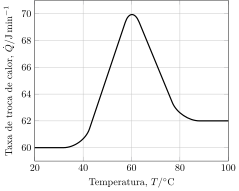
\includegraphics{images/2A44-1P.svg}
\caption{Calor por temperatura.}
\end{figure}

\begin{itemize}

\item
  \textbf{Classifique} a desnaturação como endotérmica ou exotérmica.
\item
  \textbf{Compare} a capacidade calorífica da proteína antes e após a
  desnaturação.
\item
  \textbf{Estime} a variação de entalpia da desnaturação.
\end{itemize}

\end{problem}



\begin{problem}
[2A45]Dados termodinâmicos podem ser utilizados para quantificar a
estabilidade de compostos aromáticos.

\begin{itemize}

\item
  \textbf{Determine} a entalpia de hidrogenação do cicloexeno.
\item
  \textbf{Determine} a entalpia de hidrogenação do benzeno.
\item
  \textbf{Determine} a entalpia de ressonância do benzeno.
\end{itemize}
\subsubsection*{Dados}


\begin{datalist}

\item $\Delta H_\text{f}(\ce{H2O, {l}}) = \qty{-285,83}{kJ.mol^{-1}}$
\item $\Delta H_\text{c}(\ce{cicloexano, {l}}) = \qty{-3920}{kJ.mol^{-1}}$
\item $\Delta H_\text{c}(\ce{cicloexeno, {l}}) = \qty{-3752}{kJ.mol^{-1}}$
\item $\Delta H_\text{c}(\ce{benzeno, {l}}) = \qty{-3268}{kJ.mol^{-1}}$
\end{datalist}

\end{problem}



\begin{problem}
[2A46]Considere a estrutura do fulereno,
\(\ce{C60}, \Delta H_\text{fus} = \num{1}, \Delta H_\text{vap} = \num{1}\).

\begin{figure}
\centering
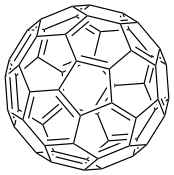
\includegraphics{images/2A46-1M.svg}
\caption{Fulereno}
\end{figure}

\begin{itemize}

\item
  \textbf{Determine} a entalpia de formação do fulereno.
\item
  \textbf{Determine} a entalpia de ressonância do fulereno.
\end{itemize}
\subsubsection*{Dados}


\begin{datalist}

\item $\Delta H_\text{f}(\ce{CO2, {g}}) = \qty{-393,51}{kJ.mol^{-1}}$
\item $\Delta H_\text{L}(\ce{C=C}) = \qty{612}{kJ.mol^{-1}}$
\item $\Delta H_\text{L}(\ce{C-C}) = \qty{348}{kJ.mol^{-1}}$
\end{datalist}

\end{problem}



\begin{problem}
[2A47]Uma massa de óxido ferroso é aquecida a \(\qty{1273}{K}\) e, em seguida,
exposta a uma mistura gasosa de monóxido de carbono e hidrogênio. O
óxido é reduzido a metal sem qualquer fornecimento adicional de energia.
O sistema perde \(\qty{4,2}{kJ}\) de calor para a vizinhança por mol de
óxido reduzido.

\textbf{Determine} a razão mínima entre as pressões parciais de monóxido
de carbono e de hidrogênio na mistura gasosa inicial, para que o
processo seja autossustentável.
\subsubsection*{Dados}


\begin{datalist}

\item $\Delta H_\text{f}(\ce{CO, {g}}) = \qty{-110,53}{kJ.mol^{-1}}$
\item $\Delta H_\text{f}(\ce{H2O, {g}}) = \qty{-241,82}{kJ.mol^{-1}}$
\item $\Delta H_\text{f}(\ce{FeO, {s}}) = \qty{-824,2}{kJ.mol^{-1}}$
\end{datalist}

\end{problem}



\begin{problem}
[2A48]A ustulação da blenda de zinco é conduzida a \(\qty{1273}{K}\) em um
reator do tipo leito fluidizado. Sulfeto de zinco misturado com sílica e
ar são adicionados em fluxo contínuo a \(\qty{273}{K}\). A reação libera
\(\qty{460}{kJ}\) de calor por mol de sulfeto a \(\qty{1273}{K}\), formando
óxido de zinco e dióxido de enxofre.

\textbf{Determine} a fração molar máxima da sílica na mistura com
sulfeto de zinco para que o processo seja autossustentável a
\(\qty{1273}{K}\).

\end{problem}



\begin{problem}
[2A49]Monóxido de carbono a \(\qty{473}{K}\) é queimado com \(90\%\) de excesso
de ar seco, a \(\qty{773}{K}\) e \(\qty{1}{atm}\). Os produtos da combustão
abandonam a câmara de reação a \(\qty{1273}{K}\).

\textbf{Determine} o calor liberado por mol de monóxido de carbono
formado.
\subsubsection*{Dados}


\begin{datalist}

\item $\Delta H_\text{f}(\ce{CO, {g}}) = \qty{-110,53}{kJ.mol^{-1}}$
\item $\Delta H_\text{f}(\ce{CO2, {g}}) = \qty{-393,51}{kJ.mol^{-1}}$
\item $C_P(\ce{CO, {g}}) = \qty{29,14}{J.K^{-1}.mol^{-1}}$
\item $C_P(\ce{CO2, {g}}) = \qty{37,11}{J.K^{-1}.mol^{-1}}$
\item $C_P(\ce{O2, {g}}) = \qty{29,36}{J.K^{-1}.mol^{-1}}$
\item $C_P(\ce{N2, {g}}) = \qty{29,12}{J.K^{-1}.mol^{-1}}$
\end{datalist}

\end{problem}



\begin{problem}
[2A50]Um carro comum possui quatro cilindros, que totalizam um volume de
\(\qty{1,6}{L}\) e um consumo de combustível de \(\qty{9,5}{L}\) por
\(\qty{100}{km}\) quando viaja a \(\qty{80}{km.h^{-1}}\). Cada cilindro sofre
\(20\) ciclos de queima por segundo. O combustível, octano, e ar são
introduzidos a \(\qty{390}{K}\) no cilindro quando seu volume é máximo,
até que a pressão seja \(\qty{1}{atm}\). Na combustão, \(10\%\) do carbono
é convertido em monóxido e o restante em dióxido. Ao final do ciclo, o
cilindro se expande novamente até o volume máximo, sob pressão final de
\(\qty{20}{atm}\).

\begin{itemize}

\item
  \textbf{Determine} a vazão de entrada de ar no motor.
\item
  \textbf{Determine} a composição da mistura gasosa de saída.
\item
  \textbf{Determine} a temperatura dos gases imediatamente após a
  combustão.
\item
  \textbf{Determine} a temperatura de saída dos gases.
\end{itemize}
\subsubsection*{Dados}


\begin{datalist}

\item $C_P(\ce{CO, {g}}) = \qty{29,14}{J.K^{-1}.mol^{-1}}$
\item $C_P(\ce{CO2, {g}}) = \qty{37,11}{J.K^{-1}.mol^{-1}}$
\item $C_P(\ce{O2, {g}}) = \qty{29,36}{J.K^{-1}.mol^{-1}}$
\item $C_P(\ce{N2, {g}}) = \qty{29,12}{J.K^{-1}.mol^{-1}}$
\item $\Delta H_\text{f}(\ce{CO2, {g}}) = \qty{-393,51}{kJ.mol^{-1}}$
\item $\Delta H_\text{f}(\ce{CO, {g}}) = \qty{-110,53}{kJ.mol^{-1}}$
\item $\Delta H_\text{f}(\ce{H2O, {g}}) = \qty{-241,82}{kJ.mol^{-1}}$
\item $\Delta H_\text{f}(\ce{octano, {l}}) = \qty{-249,9}{kJ.mol^{-1}}$
\end{datalist}

\end{problem}
\section{Gabarito}
\subsection{Nível I}


\begin{checks}
(5)
\item \MiniBox{B}
\item \MiniBox{C}
\item \MiniBox{A}
\item \MiniBox{A}
\item \MiniBox{D}
\item \MiniBox{C}
\item \MiniBox{C}
\item \MiniBox{E}
\item \MiniBox{E}
\item \MiniBox{D}
\item \MiniBox{D}
\item \MiniBox{E}
\item \MiniBox{D}
\item \MiniBox{B}
\item \MiniBox{E}
\item \MiniBox{B}
\item \MiniBox{B}
\item \MiniBox{D}
\item \MiniBox{A}
\item \MiniBox{A}
\item \MiniBox{A}
\item \MiniBox{E}
\item \MiniBox{A}
\item \MiniBox{C}
\item \MiniBox{C}
\item \MiniBox{B}
\item \MiniBox{B}
\item \MiniBox{B}
\end{checks}
\subsection{Nível II}


\begin{answers}

\item \MiniBox{C}
\item \MiniBox{D}
\item 

\begin{answers}

\item $\qty{-190}{kJ.mol^{-1}}$

\item $\qty{-286}{kJ.mol^{-1}}$

\end{answers}

\item 

\begin{answers}

\item metano: $\qty{-891,2}{kJ.mol^{-1}}$; eteno: $\qty{-1412,6}{kJ.mol^{-1}}$

\item $\qty{12}{g}$

\end{answers}

\item $\qty{4.9E15}{J}$

\item 

\begin{answers}

\item ???

\item $\num{7}$ toneladas por hora

\end{answers}

\item \MiniBox{B}
\item \MiniBox{E}
\item $\qty{6343}{kJ}$

\item 

\begin{answers}

\item ???

\item ???

\end{answers}

\item \MiniBox{E}
\item 

\begin{answers}

\item $\qty{1733}{K}$

\item $\qty{5,2}{mmol.L^{-1}}$

\end{answers}

\item \MiniBox{C}
\item \MiniBox{C}
\end{answers}
\subsection{Nível III}


\begin{answers}

\item 

\begin{answers}

\item $n = \qty{60}{mmol}$

\item $Q = \qty{8,25}{J.mol^{-1}}$.

\end{answers}

\item 

\begin{answers}

\item Endotérmica

\item Aumenta

\item $\qty{3}{J.g^{-1}}$

\end{answers}

\item 

\begin{answers}

\item $\qty{-120}{kJ.mol^{-1}}$

\item $\qty{-208}{kJ.mol^{-1}}$

\item $\qty{18}{kJ.mol^{-1}}$

\end{answers}

\item 

\begin{answers}

\item $\qty{-39,6}{MJ.mol^{-1}}$

\item ???

\end{answers}

\item $\num{1,5}$

\item 2/3

\item $\qty{-193}{kJ}$

\item 

\begin{answers}

\item $\qty{40}{L.s^{-1}}$

\item $75\%$ $\ce{N2}$, $4\%$ $\ce{O2}$, $1\%$ $\ce{CO}$, $9\%$ $\ce{CO2}$,
$11\%$ $\ce{H2O}$

\item $\qty{2000}{\degree C}$

\item $\qty{750}{K}$

\end{answers}

\end{answers}

\end{document}
